% ---- ETD Document Class and Useful Packages ---- %
\documentclass{ucetd}
\usepackage{subfigure,epsfig,amsfonts}
\usepackage{natbib}
\usepackage{amsmath}
\usepackage{amssymb}
\usepackage{amsthm}
\usepackage[toc,page]{appendix}
\usepackage[labelfont=bf]{caption}
\usepackage{rotating}
\usepackage[dvipsnames]{xcolor}
\usepackage{url}
 

%% Use these commands to set biographic information for the title page:
\title{Towards a theory of stable cell assembly formation in excitatory-inhibitory neuronal networks}
\author{Clayton W. Seitz}
\department{Graduate Program in Biophysical Sciences}
\division{Physical and Biological Sciences}
\degree{Master of Science}
\date{Winter 2021}

%% Use these commands to set a dedication and epigraph text

\epigraph{Epigraph}

\begin{document}
%% Basic setup commands
% If you don't want a title page comment out the next line and uncomment the line after it:
\maketitle
%\omittitle

% These lines can be commented out to disable the copyright/dedication/epigraph pages
\makecopyright
%\makededication


%% Make the various tables of contents
\tableofcontents
%\listoffigures
%\listoftables

%\acknowledgments
% Enter Acknowledgements here

\abstract

A central goal in computational neuroscience is to explain how spatially and temporally correlated stimuli induce spike-train correlations and the formation of stable neuronal assemblies. The dynamics of the membrane potential of a neuron embedded in a complex network is determined by many factors including network topology, homeostasis, and noise. At the same time, the network topology is not static. Synaptic plasticity allows neural circuits to guide their own topological evolution. Recently, mathematical methods for quantifying the relationship of network topology and spike train correlations based on mean-field theory and linear response theory have emerged. However, the application of these theoretical tools to structural changes, such as cell assembly formation, has been largely unexplored. At the same time, these phenomena are rarely discussed in the context of spatially-extended networks of neurons. In this thesis, I review the foundations of these theoretical models and propose (i) an important role of excitatory-inhibitory balance in assembly formation and (ii) that mean-field theory and linear response theory are capable frameworks for finding potential mechanisms of stable assembly formation.

\clearpage

\mainmatter

\chapter{Towards a theory of stable cell assembly formation in excitatory-inhibitory neuronal networks}

The thesis has been divided into two primary sections following the Introduction. The first section paints a broad picture of the theoretical techniques that can be used to analyze spike train cross correlations as well as their mathematical connections to network structure. In addition, this section summarizes the mathematical machinery that can relate network dynamics to synaptic plasticity. The second section contains the results from a set of rudimentary simulations which form the basic substrate for further analyses. The scope of these simulations is necessarily narrow. Significant computational advances are needed in order for the simulations to fully connect with the theory.

\section{Introduction}

Complex systems are ubiquitous in nature yet our scientific efforts have thus far only begun to gain traction on their governing principles. Complex systems often exihibit behaviors that simply cannot be explained by any of the components in isolation but rather arise from their interactions, bringing emergent phenomena into the focus of modern science. The brain exemplifies this complexity, thought to consist of billions of noisy neurons, yet the dynamics of these neurons simulataneously maintain an order evident in the stability of our sensory percepts. How functional brain states emerge from the interactions of dozens, perhaps hundreds, of brain regions, each containing its own complex subnetworks, remains a complicated problem. It is well accepted that information processing in the brain like sensory, motor, and cognitive functions are carried out by correlated spiking of individual neurons, formally referred to as a \emph{population code}. However, is a great challenge to understand how this correlation structure relates to the statistics of sensory stimuli, how it forms, and how it is maintained. 

Early models of neural networks were often deterministic; however, an increasing body of experimental data suggests that neurons, synapses, and systems of neurons are inherently stochastic (Buesing, 2011). The enormous number of degrees of freedom of just a single cell due to millions of unreliable ion channels and synaptic machinery demands a stochastic model for network dynamics. Indeed, it has been argued that the variability in neural responses to stimuli and the irregularity of spike-timing owe their origins, in part, to noise in the synaptic integration process (Azouz, 1999). The mechanisms by which networks can exhibit stable dynamics, correlated states, and stable cell assembly formation amidst this stochasticity are important issues. 

Some of the most mature models of network dynamics describe the averages of dynamical quantities or involve the solution of stochastic differential equations. The former technique is realized by a mean-field theory of network dynamics which replaces synaptic currents by their average values - a valid approximation in the limit of very large networks (Vreeswijk 1999). The method was originally developed in simple excitatory-inhibitory random network models but has been more recently extended to networks where synaptic probabilities are a function of space (Rosenbaum 2017). In the mean-field framework, one can prove the existence of a \emph{balanced state} in which excitation and inhibition cancel eachother. The existence of such a state is thought to contribute to the irregularity of spike-timing observed \emph{in-vivo} and neuronal information processing at large. Interestingly, in the balanced state, the spatial structure of spike-train correlations was shown to have a distinct spatial profile, similar to reported measurements in macaque V1 (Rosenbaum 2017). Both theory and experiment show that nearby cells tend to be positively correlated, moderately distant cells negatively correlated, and distant cells show weak correlation. At any rate, proving the existence of a balanced state often places rigid requirements on the network topology, which are not reminiscent of the synaptic weight distribution in real neural networks. 

Another class of methods, sometimes referred to as population density methods, predict the membrane potential distribution of an ensemble via a diffusion approximation i.e. by solving the Fokker-Planck equation. The Fokker-Planck formalism has proven quite useful and naturally lends itself to the description of ensembles of neurons. However, its analytical solution is known only for relatively simple networks and simple integrate and fire neuron models. More complex single neuron models, such as exponential integrate and fire (EIF) models, require special numerical treatment. Also, the Fokker-Planck equation is generally used as a low-dimensional description of the network and imposes strong assumptions on its topology such as sparsity (Brunel 2000). If used in isolation, it is limited to special cases and precludes the analysis of more complex dynamical regimes. However, the Fokker-Planck formalism can be used as a first approximation to network dynamics, and refinements of that prediction can be subsequently added. For example, in the linear response framework, a first approximation of network dynamics can be found by uncoupling the neurons and solving the Fokker-Planck equation. Corrections to that first approximation are then found by using uncoupled firing rates to find spike-train power spectra, which are then propagated through the network according to its topology. In short, this technique can be used to make predictions for more complex network topologies than those often used in a mean-field framework and can be extended to make predictions of the network topology that results from the underlying spike-train statistics (Ocker 2015; 2017). 

In his famous neurophysiological postulate, Donald Hebb first proposed a cellular mechanism for the self-organization of networks of neurons. Hebb suggested that repeated stimulation of specific receptors of sensory signals would lead slowly to the formation of a \emph{cell assembly} and these structural changes would constitute a representation or imprint of an internally or externally generated sensation e.g., an image or idea (Hebb 1949). This process, which is now known as a \emph{heterosynaptic} plasticity mechanism, is argued to be driven by the frequency and temporal order of action potentials. On the other hand, experimental evidence and the results of computational studies suggest that a complex orchestration of different types of plasticity mechanisms are necessary for stable formation of cell assemblies (Kumar 2014; Zenke 2015). In this thesis, it will be argued that the spatial correlation structure predicted by mean-field theory for balanced spatially-extended networks could result in spatially-dependent plasticity. The non-monotonicity of the spatial-dependence of spike-train correlations could have important implications for synaptic competition and stable assembly formation. Deviations from the balanced state predicted by mean-field theory could then be addressed using linear response techniques, which have been recently generalized to accomodate for slow changes in network topology (Ocker 2015).

\clearpage
\section{Literature Review and Theoretical Foundations}


Recent experimental advances permit the recording of spike trains of many neurons simultaneously \emph{in-vivo}. These experiments have revealed that significant spatial and temporal correlations exist in the timing of spikes by individual neurons, bringing the role of correlations in neural computation into question. Often, such studies are necessarily contextual - correlations must be interpeted in the context of known stimulus drive, learning or experience, or changes in behavioral context (Cohen 2011). Interpretation of such correlations has been a fruitful exercise; however, it is also important to understand the properties of neuronal networks that give rise to them such as topological parameters and synaptic plasticity. For pairs of neurons, correlations are often quantified according to the cross-correlation function of their spike trains (Ostojic 2009). The profile of this cross-correlation function is dependent on several factors including direct synaptic wiring (Csicsvari 1998) or common and potentially correlated inputs. Although cross-correlation analysis of experimental recordings can provide substantial information regarding circuit architecture, relating the correlations of spike trains to the underlying circuit architecture remains a long-standing problem in computational neuroscience. To approach this problem, simulations of networks of model neurons are often used (see Fig (1.1)). In these simulations, network parameters are tuned to examine the resulting correlation structure of spike trains with the hope of inverting the model for comparison with \emph{in-vivo} recordings. 

%\clearpage
\begin{figure}[t!]
\centering
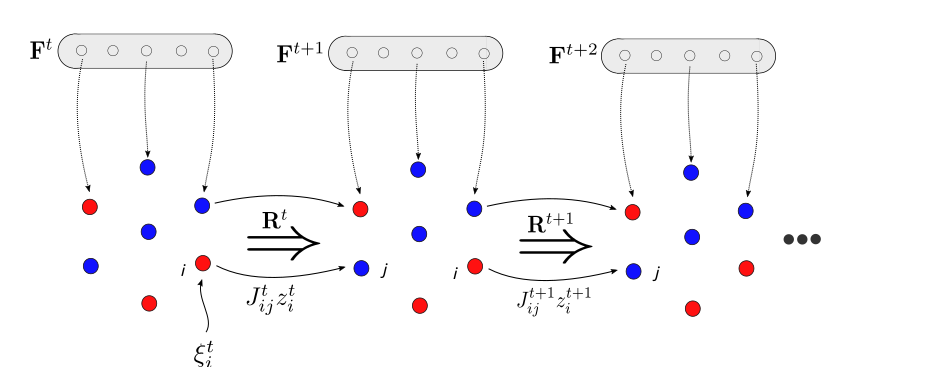
\includegraphics[width=175mm]{figure-1}
\caption{Cartoon of a excitatory-inhibitory neural network receving a time-dependent feedforward current $F(t)$, feedback current $R(t)$, and synaptic noise $\xi(t)$. Excitatory neurons are shown in red and inhibitory neurons shown in blue. Synaptic current is drawn to be instantaneous and syanptic weights $J_{ij}$ are not functions of time. Feedforward inputs could be weighted Poisson processes where $F$ defines the rates, for example.}
\end{figure}

In addition to non-trivial correlations in their spike timing, neurons in cortical networks tend to exhibit highly irregular time intervals between spikes. The stochasticity in spike timing has can be attributed to cellular and sensory noise (Faisal 2008), or alternatively to network-scale mechanisms such as excitatory-inhibitory balance (Vreeswijk 1996, 1998). Amidst this irregularity, our understanding of spike correlations are further complicated by the nonlinear dynamics of recurrent network models (Baker 2019; Tetzlaff 2008, 2012; Doiron 2016; Ocker 2017). It is common to tame this complexity by making suitable combinations of assumptions regarding the statistics of network stimuli, the mechanism of neuron-neuron interactions, or the statistics of synaptic connectivity. For example, in the mean-field approximation strong assumptions are often made regarding the synaptic connectivity in order to estimate the mean value of synaptic currents. As a rule, the postsynaptic current to a neuron embedded in a spiking network model consists of two components: feedforward $F(t)$ and feedback $R(t)$:

\begin{align}
I(t) = F(t) + R(t) + \xi(t)
\end{align}

Notice the additional noise term $\xi(t)$, which serves to capture channel noise or noise in the synaptic integration process. This is frequently taken to be delta-correlated Gaussian noise. A variety of models for the integration of this current into a stateful membrane potential exist. Here, we are particularly interested in non-linear integrate and fire models which are described by the Langevin equation

\begin{equation}
\tau\dot{V}(t) = g_{\ell}(E - V) + g_{\ell}\cdot \psi(V) + I(t)
\end{equation}

where $g_{\ell}$ is a leakage conductance and $E$ its reversal potential. An important case of (1.2) is the exponential integrate and fire (EIF) model where $\psi(V) = \Delta_{T}\exp\left(\frac{V-V_{T}}{\Delta_{T}}\right)$ is a spike generating current. This model is an extension of the standard linear integrate and fire models which more accurately captures the initial dynamics of spike-generating sodium channels (Richardson 2007). To produce spiking behavior, the membrane potential is passed through a thresholding function which produces spike trains. Spike trains are represented as sums over delta functions

\begin{equation}
z(t) = \sum_{i} \phi(t) * \delta(t-t_{i})
\end{equation}

where the variable $z(t)$ is sometimes called the \emph{observable state} of a neuron and is computed from the voltage according to $z(t) = H(V(t) - V_{\mathrm{th}})$ where $H$ is the Heaviside step function and $V_{\mathrm{th}}$ the firing threshold. The time-dependent firing rate of a neuron is given by averaging the above spike train across multiple realizations $r(t) = \langle z(t) \rangle$. In addition, to avoid instantaneous synapses, $z(t)$ can be convolved with the synaptic kernel $\phi(t)$, which is often taken to be a decaying exponential, as is done in later sections. Immediately after firing an action potential, the membrane potential is reset to a resting value $V_{\mathrm{re}}$ and it is held there for a refractory period $\tau_{\mathrm{ref}}$. Of course, in a network, (1.3) is directly related to the feedback current in (1.1) by 

\begin{equation}
R_{i}(t) = \sum_{j} J_{ij}\cdot \phi(t) * \delta(t-t_{i})
\end{equation}

Ultimately, our goal is to understand the origins of correlations or lack thereof in the variable $z(t)$ across a population of neurons. A natural starting point is to consider the case where spike-trains are uncorrelated, which can occur in the presence of balanced excitation and inhibition.

\subsection{The mean-field approximation in logical networks}

A network model $J$ will be called \emph{logically connected} when connection probabilities are not a function of spatial coordinates. Therefore, a network will be called \emph{spatially connected} or \emph{spatially extended} when they are. The remainder of this section deals with the former class of networks. As mentioned, theoretical work has proposed that the irregular inter-spike intervals observed in experiments can be explained by approximate balance of excitatory and inhibitory synaptic currents (Vreeswijk, 1996). In this balanced regime, the timing of the firing of cells is sensitive to the relatively small fluctuations in their total synaptic input because the excitatory and inhibitory inputs cancel each other (Amit, 1995). Also, excitatory and inhibitory balance has been theoretically shown to enhance the sensitivity of a cell to fluctuations on a timescale much smaller than a typical integration time constant (Vreeswijk, 1996; Tian 2020). Interestingly, model neurons optimally detect temporal information when the average membrane potential is one standard deviation of the noise below threshold, a phenomenon known as stochastic resonance (Plesser, 2000; Kempter, 1998). A general framework for generating balanced logical networks has been developed. In the following paragraphs, the terminology and mathematical machinery introduced in (Vreeswijk 1996) and later used by (Renart 2010; Rosenbaum 2017) and others will be described.

A network model is called \emph{sparse} if the probability of a connection between a neuron in a population $\alpha$ and neurons in a population $\beta$ scales with the network size $N$ according to $p_{\alpha\beta} \sim \mathcal{O}(1/N)$. As a result, the degree $K$ of a neuron does not depend on the scale of the network or $K \sim \mathcal{O}(1)$. In contrast, we then say that a network is \emph{dense} if the above connection probability scales as $p_{\alpha\beta} \sim \mathcal{O}(1)$ such that the degree of a neuron scales as $K \sim \mathcal{O}(N)$. Moreover, the efficacy of a synaptic connection between populations $\alpha$ and $\beta$ is said to be \emph{strong} if $J_{\alpha\beta} \sim \mathcal{O}(1)$ and \emph{weak} coupling occurs when $J_{\alpha\beta} \sim \mathcal{O}(1/\sqrt{N})$. If a network is both dense and weakly coupled, this choice of scaling for $J_{\alpha\beta}$ and the degree $K$ results in the total synaptic input to a neuron scaling as $\mathcal{O}(\sqrt{N})$. In this case, it is possible to parameterize the network such that fluctuations in the synaptic input currents saturates to a value of the order of the spiking threshold, in the limit of large $N$ (Vreeswijk, 1996; Renart 2010; Rosenbaum 2017).  

The scaling of synaptic inputs outlined above is a critical step towards finding the balanced state. To see this, consider the total synaptic current injected into a neuron $i$ within a population $\alpha$, decomposed into its feedfoward and recurrent components

\begin{align}
I_{i}^{\alpha}(t) &= F_{i}^{\alpha}(t) + R_{i}^{\alpha}(t)\\
&= F_{i}^{\alpha}(t) + \sum_{\beta}\sum_{j} \frac{J_{ij}^{\alpha\beta}}{\sqrt{N}}(\phi * z^{\beta}_{j}(t))
\end{align}

Again, for the sake of generality, the spike-train $z^{\beta}_{j}(t)$ is convolved with a synaptic kernel $\phi$, determining the shape of the post-synaptic potential induced by a spike. In the mean-field approximation we replace the current in each term of the sum over $j$ in (1.2) by its average value, which is a valid approximation in the limit $N\rightarrow\infty$ (Vreeswijk 1996). For the sake of simplicity, take $\phi = \delta(t)$, and the observable state $z^{\beta}_{j}(t)$ is replaced by the average firing rate of a neuron in population $\beta$ multiplied by the probability of a connection $p_{\alpha\beta}$

\begin{align*}
\langle I_{i}^{\alpha}(t)\rangle &= \langle F_{i}^{\alpha}(t)\rangle + \langle R_{i}^{\alpha}(t)\rangle\\
&= \langle F_{i}^{\alpha}(t)\rangle + \sqrt{N}\sum_{\beta}j_{\alpha\beta}p_{\alpha\beta}r_{\beta}
\end{align*}

with $j_{\alpha\beta} = J_{\alpha\beta}\sqrt{N}$. Notice that the average value of the recurrent contribution to the synaptic current indeed saturates for large $N$. Writing the above equation explicitly for a neuron in an excitatory-inhibitory network i.e. $\alpha, \beta \in \{e, i\}$

\begin{align}
\langle I_{j}^{e}(t)\rangle &= \langle F_{j}^{e}(t)\rangle + \sqrt{N}\left(j_{ee}p_{ee}r_{e} + j_{ie}p_{ie}r_{i}\right)\\
\langle I_{k}^{i}(t)\rangle &= \langle F_{k}^{i}(t)\rangle + \sqrt{N}\left(j_{ii}p_{ii}r_{i} + j_{ei}p_{ei}r_{e}\right)
\end{align}

If we require that, in the mean-field limit $N\rightarrow\infty$, the average current vanishes and that $\langle F_{j}^{\alpha}(t)\rangle \sim \mathcal{O}(\sqrt{N})$ we have the following matrix equation relating the mean field firing rates to the synaptic weights and average feedforward current

\begin{align}
\begin{pmatrix}
j_{ee} & j_{ie}\\
j_{ei} & j_{ii}
\end{pmatrix}
\begin{pmatrix}
r_{e}\\
r_{i}
\end{pmatrix}
= 
-\begin{pmatrix}
\langle F_{j}^{e}\rangle\\
\langle F_{k}^{i}\rangle
\end{pmatrix}
\end{align}

Assuming that the above matrix is invertible, we have the following solution

\begin{align}
\underset{N\rightarrow \infty}{\mathrm{lim}}r_{e} = \frac{\langle F_{j}^{e}\rangle j_{ii}-\langle F_{k}^{i}\rangle j_{ie}}{j_{ei}j_{ie} - j_{ee}j_{ii}}
\end{align}

\begin{align}
\underset{N\rightarrow \infty}{\mathrm{lim}}r_{i} = \frac{\langle F_{k}^{i}\rangle j_{ee}-\langle F_{j}^{e}\rangle j_{ei}}{j_{ei}j_{ie} - j_{ee}j_{ii}}
\end{align}

For positive solutions for the above firing rates and for the above matrix to be invertible we have the rather loose condition $\langle F_{j}^{e}\rangle/\langle F_{k}^{i}\rangle > j_{ie}/j_{ii} > j_{ee}/j_{ei}$ and we recover the condition given in (Rosenbaum 2014; Rosenbaum 2017; Akil 2021). Notice that the parameters specific to the neuron model do not enter into the equation above. 

The technique used above has also been extended to account for correlations in neural spike trains arising from correlation in synaptic currents. Indeed, this method has been successfully generalized to logically coupled networks with many populations as well as networks which are spatially extended (Rosenbaum 2017). It has also been applied to networks receieving temporally correlated stimuli (Baker 2019). However, proving the existence of a balanced state simultaneously requires some rather harsh assumptions about the synaptic weights. Weight distributions observed in experiments are unimodal and long-tailed (Perin 1997; Song 2005). Also, the method is not readily generalizable to plastic networks, although deviations from the balanced state under a spike-timing dependent plasticity rule have been described (Akil 2021). Nevertheless, the balanced state is a natural starting point for simulations, as it successfully captures the spike-timing irregularity observed \emph{in-vivo}.

\subsection{The diffusion approximation and linear response}

Another method used to predict the dynamics of excitatory-inhibitory networks utilizes the so-called \emph{diffusion approximation}. If the presynaptic partners of a neuron are each described by an inhomogeneous point process, the total synaptic current $I(t)$ can have complex statistics depending on presynaptic firing rates and their correlations. However, in some special cases, such as when presynaptic firing rates are large, synaptic currents are safely assumed to be Gaussian (Richardson 2007). To begin to examine this, we combine equations (1.1), (1.2), and (1.4) for a single neuron $i$ to give 

\begin{equation}
\tau\dot{V}_{i}(t) = g_{\ell}(E_{i} - V_{i}) + g_{\ell}\cdot\psi(V_{i}) + F_{i}(t) + \xi(t) + \sum_{j} J_{ij}\cdot \left(\phi(t) * z_{j}(t)\right)
\end{equation}

where it is assumed that $\xi(t)$ is a delta correlated white noise i.e. $\langle\xi_{i}(t)\xi_{j}(t)\rangle = \delta(i-j)$ and $\langle\xi_{i}(t)\xi_{i}(t')\rangle = \delta(t-t')$. When expressed for all neurons $i$ simultaneously, the above becomes a high-dimensional stochastic differential equation, which in general is difficult to work with. Rather than solving (1.12) directly, in the linear response approximation a realization of the spike train $z_{i}(t)$ is approximated as a sum of two terms which represent the spike train in the absence of feedforward and feedback currents and a linear filter of the feedback currents

\begin{align}
z(t) \approx z_{0}(t) + (A * R)(t) 
\end{align}

If averaged over many realizations, the above instead becomes an expression for the firing rate. The equation above is the central claim made by a linear reponse theory of network dynamics. For simplicity, it is natural to start with the case where $F_{i}(t)$ is itself a Gaussian white noise independent of the intrinsic noise. Therefore, the intrinsic noise $\xi(t)$ and the feedforward stimulus can be absorbed into a single noise term. Then, $z_{0}(t)$ is a realization of a spike train in the absence of feedback when its stimulation is a sum of feedforward and intrinsic noise. In the frequency domain (1.13) for a particular neuron reads (Linder 2005; Trousdale 2012)

\begin{align}
z_{i}(\omega) = z_{i}^{0}(\omega) + A(\omega)\left(\sum_{j}J_{ij}(\omega)z_{j}(\omega)\right)
\end{align}

The matrix $J(\omega)$ is the frequency domain representation of the synaptic connectivity matrix after convolution with the synaptic kernel and $A(\omega)$ is the transfer function or linear response function in the frequency domain. This equation can then be rewritten in matrix form to give the frequenty domain representation of the spiking activity across all neurons in the population simultaneously

\begin{align}
z(\omega) = z_{0}(\omega) + A(\omega)J(\omega)z(\omega)
\end{align}

The result above can then be solved for $z(\omega)$ to give 


\begin{align}
z(\omega) = \left[I-A(\omega)J(\omega)\right]^{-1}z_{0}(\omega)
\end{align}

where $I$ is the identity matrix. Making the substitution $\Delta(\omega) = \left[I-A(\omega)J(\omega)\right]^{-1}$, the expression above can then be used to obtain the cross-spectrum (and therefore the cross-correlations) of two spike trains $z_{i}(\omega)$ and $z_{j}(\omega)$ for all possible pairs. 

\begin{align}
\langle z(\omega)z^{*}(\omega)\rangle &= \langle \Delta(\omega)z_{0}(\omega)z_{0}^{*}(\omega)\Delta^{*}(\omega)\rangle\\
&= \Delta(\omega)C^{0}(\omega)\Delta(\omega)^{*}
\end{align}

The above result is the matrix of cross spectra across the population $C(\omega)$ in the absence of correlated inputs. The matrix $C^{0}(\omega)$ is a diagonal matrix with $C_{ii}^{0}(\omega)$ being the spectrum of the spike train of a neuron $i$ when the neurons are decoupled. The interpretation of equation above is that we can first find a matrix of cross-spectra when neurons are uncoupled $C^{0}(\omega)$ and then solve (1.18) to estimate the full cross-spectra in the network. This proves very useful for examaple when analyzing the effects of the topology $J$ on the matrix $C(\omega)$ (Trousdale 2012; Ocker 2015). In any case, the matrix $C^{0}(\omega)$ and the linear response function $A(\omega)$ are still unknown, and must be found. The assumption that feedforward inputs and intrinsic noise are white permits the use of a diffusion approximation to find the individual rates and therefore the spectra $C_{ii}^{0}(\omega)$. Under conditions in which a diffusion approximation applies, the Kramers-Moyal expansion can be reduced to the Fokker-Planck equation. The Fokker-Planck equation for the stochastic integrate and fire model given in (1.12) in the absence of feedback is

\begin{align}
\frac{\partial P}{\partial t} &= \frac{\sigma^{2}}{2}\frac{\partial^{2}P}{\partial V^{2}} + \frac{\partial}{\partial V}\left(\frac{V-E-\psi}{\tau}P\right)
\end{align}

where $\sigma^{2}$ is the variance of the Gaussian input current. We can solve the Fokker-Planck equation above to estimate the firing rates of neurons when they are uncoupled and therefore estimate $C^{0}(\omega)$. However, the solution for non-linear integrate and fire models frequently requires numerical integration of (1.19) to find the stationary density over the membrane potential and to estimate steady state firing rates (Richardson 2007). Similarly, the frequency response $A(\omega)$ can be found by using the solution to the Fokker-Planck equation under a weak sinusoidal perturbation to the synaptic current (Richardson 2007; 2009). A more detailed description of these procedures is given in the Methods. It should be noted that a diffusion approximation is not limited to the case where neurons are uncoupled. It can also be used when synaptic connectivity is sufficiently sparse, and the probability of two neurons sharing synaptic inputs vanishes. In that case, the synaptic current to a neuron can be guaranteed to follow a normal distribution, per the central limit theorem (Brunel 2000).  It is also a valid assumption when the population fires asychronously and the feedback $R(t)$ is a sum over independent processes, even in dense networks (Tian 2020).

Furthermore, the solution for $C(\omega)$ given in (1.18) has been derived in an alternative fashion by using an iterative approach (Trousdale 2012). This approach is highly valuable as it builds an estimate of $C(\omega)$ by considering paths through a recurrent network of increasing length. Here, a very abstract description of approach will be given and most of the mathematical details are deferred to the original text (Trousdale 2012). Intuitively, the spike-train correlation between a pair of cells can be estimated from the activity of presynaptic cells $n$ synapses away from the cells under consideration. We expect then to improve our estimate of $C(\omega)$ for large values of $n$. For the simplest case, when $n=0$, the neurons are uncoupled and we have $C(\omega) = C^{0}(\omega)$. When $n=1$, we consider only the nearest neighbors in calculating the cross-correlation between neurons $i$ and $j$ and improve on the uncoupled estimate $C^{0}(\omega)$. It can be proven that in the limit $n\rightarrow\infty$ this iterative procedure also yields (1.18). Trousdale et al. further generalized their iterative approach to give the matrix of cross-spectra in the case were feedforward inputs can have non-trivial correlations


\begin{align}
C(\omega) &= \Delta(\omega)\;C^{0}\;\Delta^{*}(\omega) + \Delta(\omega)\;A(\omega)C^{\mathrm{ext}}(\omega)A^{*}(\omega)\;\Delta^{*}(\omega)
\end{align} 

This is a very important result as it provides a mechanism for probing the transfer of feedforward correlations to the correlations of spike trains. The first term represents the component of the cross spectra from internally generated correlations. The second term is the component that is caused by correlations in the feedforward input. Perhaps the feedforward inputs $F(t)$ are drawn from a multivariate gaussian distribution i.e. $F(t) \sim \mathcal{N}(\mu,\Sigma)$ and we would like to know how $\mu$ and $\Sigma$ affect network dynamics. Ultimately, the linear theory provides a direct mechanism for solving for the cross-covariance of spiking in the population in terms of the synaptic coupling matrix, for arbitrary network topologies. Interestingly, previous analyses have used the above relations to describe the dynamics of motifs under synaptic plasticity when feedforward input is uncorrelated (Ocker 2015). The theory above is very powerful and has several applications. For present purposes, a particularly interesting application would be an examination of the degree of stability of cell assembly formation under different classes of plasticity rules. 

It should be noted that models which are dependent on a diffusion approximation, like a linear response theory, have limitations. In particular, the integration of temporally correlated presynaptic spike trains can result in non-trivial two-point correlation functions that are not well-described by a Gaussian white noise process (Moreno-Bote 2008). This has been noted before, in studies of the numerical solution of the Fokker-Planck and master equations which recognized a disparity between the diffusion approximation and full shot-noise stochastic dynamics (Nykamp 2001). Recordings \emph{in-vivo} also have shown the synaptic fluctuations can have significant non-Gaussian properties (DeWeese 2006). In any case, the diffusion approximation and solution of the Fokker-Planck equation can describe important biophysical properties of neuronal response. For example, synaptic filtering, activation of non-linear voltage-gated currents, and non-linear response properties at the onset of a spike (Richardson 2007).

\subsection{Reshaping network structure with synaptic plasticity}

Activity dependent modification of synaptic efficacy or the formation of new synapses is the putative basis of learning and memory formation. The chaining of cellular assemblies that form as a result of synaptic plasticity are thought to provide a structural basis for many cognitive processes such as memory retrieval, reasoning, and planning (Buzaki 2010). Recent neurobiological advances have provided substantial insight on the biochemical and biophysical mechanisms of plasticity. However, the formation of functional circuits and their stability amidst ongoing network dynamics remains unclear.

Plasticity mechanisms are highly diverse and occur over a wide range of time scales: from milliseconds to hours to days (Zenke 2015). For example, short-term synaptic plasticity (STP) is thought to provide a richer set of network responses to stimuli without permanently altering the circuit architecture. For example, repeated stimulation of a presynaptic cell can cause a transient accumulation of Ca2+ in the presynaptic terminal, which has been proposed as a mechanism for short-term memory (Mongillo 2008). Calcium ions elevate the probability of neurotransmitter release due to its proposed interaction with the biochemical machinery involved in synaptic vesicle exocytosis. Other short term changes in synaptic efficacy can occur such as the facilitation or depression based upon the temporal characteristics of the stimulus. Paired-pulse experiments have yielded evidence that tetanic stimulation can result in inactivation of voltage-dependent sodium and/or calcium channels or depletion of the release ready pool of synaptic vesicles at the presynaptic terminal. Synaptic efficacy can alternatively be lowered by the release of biochemical neuromodulators which can interact with the synaptic machinery to inhibit the release of neurotransmitter into the synaptic cleft. Thus, these neuromodulators can also play a role in facilitation or depression in STP.

It is well-accepted that neural circuits also possess the mechanisms for long term changes in synaptic strength formally referred to as long term potentiation (LTP) and long term depression (LTD). The brain encodes internally and externally generated stimuli as spatiotemporal patterns of action potentials and long-term modifications to such patterns via changes in synaptic transmission provide a feasible mechanism for the storage of information. In other words, permanent or semi-permanent changes in synaptic weights alter the spatiotemporal response of population of neurons to stimuli and therefore provide a method for long term memory formation. Since its inception by Cajal, this idea has been rigorously tested, for example in the CA1 region of the hippocampus (Whitlock et al. 2006). The modification of spatiotemporal characteristics of the neural response to stimuli suggest that evidence for plasticity can be found in the correlation structure of neural spike trains.

Early work on synaptic plasticity at the cellular level demonstrated that LTP in slices of hippocampal tissue could occur as a result of tetanic stimulation of a post-synaptic cell (Bliss 1973) while low frequency stimulation can drive LTD. If many fibers are stimulated at frequencies exceeding $50\text{Hz}$, postsynaptic potentials can increase by 50-100\% (Sejnowski 1989). Additional research expanded upon this observation, noting that temporal correlation of presynaptic and postsynaptic spiking affected plasticity. In particular, strong temporal correlation of presynaptic and postsynaptic firing rates on a timescale of $\pm 100 \text{ms}$ can give rise to LTP. The discovery of these phenomena has resulted in the proposal of a wide variety of different plasticity rules which fall under the umbrella of `Hebbian' learning rules. Hebbian learning rules have been broadly defined as rules in which the change in synaptic efficacy depends only on pre-synaptic and post-synaptic variables and that changes to the synapse depend interactively on these two variables and not separately (Sejnowski 1989).  Additionally, Hebbian learning rules are \emph{causal} in that LTP occurs when the presynaptic neuron contributes to the firing of the postsynapic cell and LTD occurs otherwise.

Additional efforts demonstrated that the sign and magnitude of LTP and LTD depend on the order and delay of presynaptic and postsynaptic action potentials, on a time scale of $10\text{ms}$ (Markram 1997), later named spike timing dependent plasticity (STDP) (Song 2000). In the original formulation of Hebbian STDP, LTP can occur when presynaptic spikes lead postsynaptic spikes by $\sim 20\mathrm{ms}$ and LTD can occur when postsynaptic spikes lead presynaptic spikes by $\sim 20-100\mathrm{ms}$ (Markram 1997; Bi and Poo 1998; Celikel 2004; Feldman 2012). However, plasticity does not only depend on spike timing, but also on other factors such as firing rates, and synaptic cooperativity, and postsynaptic voltage (Makram 1997). Therefore, findings indicate that STDP is part of a broader class of plasticity rules and may be viewed as the spike timing component of a multifactor plasticity rule (Feldman 2012).

Furthermore, the biochemical mechanism of synaptic plasticity is regulated by the release of neurotransmitters by the presynaptic cell and/or by modifying the density of receptors at the postsynaptic membrane (Sumi 2020). Indeed, it is widely believed that presynaptic release of glutamate results in activation of AMPA receptors and subsequent depolarization of the post-synaptic membrane. Membrane depolarization then activates the N-methyl-D-aspartate receptor (NMDAR), which is permeable to Ca2+ which is a prefactor in a biochemical cascade resulting in the trafficking of AMPA receptors to the postsynaptic membrane. High elevations in Ca2+ concentrations in the presynaptic cell are believed to result in an increased density of AMPA receptors at the postsynaptic membrane and in elevated excitatory postsynaptic potentials (EPSPs) thereby providing a mechanism for LTP (Sumi 2020). In summary, LTP versus LTD induction is determined by the magnitude and time course of calcium flux (Lisman 1989). When the presynaptic cell fires first, the EPSP produces a strong NMDAR calcium flux while while when the postsynaptic cell fires first, this flux is weak. On the other hand, LTD has not been shown to occur soley due to minor elevations in Ca2+ concentrations, but is thought to result from a retrograde signaling mechanism in which presynaptic transmitter release probability is decreased (Nabavi 2013).

Beyond spike-timing dependent plasticity, other plasticity mechanisms have been observed experimentally. In the hippocampus, non-Hebbian heterosynaptic LTD alongside LTP was described shortly after the phenomenon of LTP was discovered (Lynch 1977). The Hebbian mechanisms or \emph{associative mechanisms} discussed above are termed homosynaptic mechanisms, as they depend on both pre- and post-synaptic activity. There are also heterosynaptic mechanisms which depend on only the state of the post-synaptic neuron and are thought to exist to counteract chaotic dynamics introduced by Hebbian-type rules and to balance synaptic changes. Hebbian homosynaptic learning rules, by definition, potentiate (depress) synapses with positive feedback, meaning that increasing (decreasing) synaptic efficacy will promote further potentiation (depression). For example, The standard doublet STDP model gives rise to splitting of synaptic weights, producing a bimodal distribution; however, weight distributions observed in experiments are unimodal and long-tailed (Perin 1997; Song 2005). The result is the overexcitability of some neurons and silencing of others making network dynamics unstable. Induction of LTD at high firing rates of the postsynaptic neuron is a candidate for an intrinsic stabilization mechanism (Kempter 2001). Also, it has been recent suggested that rate-dependent terms in the synaptic learning rule can stabilize motif configurations (Ocker 2015). Ultimately, it is thought that a push-pull mechanism exists in which homosynaptic LTP prevents the network from falling silent at low firing rates while heterosynaptic LTD prevents the runaway dynamics at high firing rates.

Understanding the stable formation and maintenance of cell assemblies is an additional goal of synaptic plasticity research. From a n\"{a}ive point of view, a cell assembly could form if a subset of a neuron's inputs were to potentiate while other inputs depress. However, for this to occur both groups should be repeatedly activated either with highly specific patterns to promote LTP or LTD, respectively (Chistikova 2014). This could then limit network stability to special sequences of input patterns while we expect that plasticity mechanisms exist to promote stability under a variety of input stimuli. Moreover, experiments involving intercalated neurons of the amygdala have demonstrated that LTP induction with high-frequency stimulation can simultaneously result in heterosynaptic depression (Royer 2003). Conversely, LTD induction with low-frequency stimulation was also shown to induce LTP. These observations indicate the existence of intracellular signaling that would provide synapses with `awareness' of eachother. Learning rules which depend on the post-synaptic firing rate would produce a similar result, although often these rules do not perform selective potentiation or depression. That is, synaptic weights are normalized without regard to which synapses can be blamed for chaotic or silent neuron states. In circuits with highly regular organization of the inputs, such as the hippocampus or amygdala, the onset of LTP can induce weaker LTP at nearby inputs while concurrently inducing heterosynaptic LTD at more distant inputs, while the magnitude of LTD decreasies with distance (Royer 2003).

The experiemental observations discussed suggest that balanced LTP and LTD may be a powerful mechanism of for synaptic normalization and synaptic competition. Thus, several computational studies incorporating more realistic forms of synaptic plasticity with conductance based neuron models have surfaced (Zenke 2015; Kumar 2014). Many have incorporated a balance between excitation and inhibition to capture the irregular activity of cortical networks, but stable formation of cell assemblies is difficult to achieve. This shortcoming could, in part, be due to the tendency of STDP to lead to pathological behavior in balanced networks (Morrison 2007). The introduction of homeostatic mechanisms such as normalization of total conductance alongside inhibitory STDP to control the firing rate of excitatory neurons has been used to inhibit pathological activity in the balanced regime (Kumar 2014). 

Returning to the theoretical discussion, in a plastic network the synaptic weights (conductances) are functions of time. Thus a more general form of (1.4) reads

\begin{align*}
I_{j}^{\alpha}(t) &= \sum_{\beta}\sum_{i} g_{ij}^{\beta}(t)(E_{\beta} - V_{j})\\
&= \sum_{\beta}\sum_{i}J_{ij}^{\alpha\beta}(t)\left(\phi\;*\;z_{i}(t)\right)(E_{\beta} - V_{j})
\end{align*}

Biologically, excitatory conductances such as AMPAR/NMDAR would be under the control of an excitatory neurotransmitter e.g. glutamate while inhibitory conductances regulated by perhaps gamma-aminobutyric acid (GABA). Notice that the time-dependence of $g^{\alpha}$ can then be given by the convolution of an excitatory presynaptic spike train $z_{i}(t)$ or inhibitory spike train $z_{k}(t)$ with an appropriate synaptic kernel $\phi$. The synaptic plasticity rule is then a rule for the time-derivative $\dot{J}^{\alpha\beta}_{ij}$.


The cellular machinery of plasticity mechanisms described above highlights the importance of spike-time correlations, generated by recurrent feedback or feedforward projections, in determining the evolution of synaptic weights. A classic derivation of the evolution of synaptic weights for interacting Poisson processes was given in (Kempter 1999). This result is an important starting point for later analysis. Consider the total change in the synaptic weight between neurons $i$ and $j$ as $\Delta J_{ij} = J_{ij}(t+\Delta t) - J_{ij}(t)$ in a time interval $\Delta t$. Consider the very general rule for a single spiking neuron $i$ receiving many inputs indexed by $j$
\begin{align*}
\dot{J_{ij}} = a_{0} + a_{i}z_{i}(t) + a_{j}z_{j}(t) + F(z_{i}(t),z_{j}(t))
\end{align*}


for a yet unknown function $F$, which could be a STDP rule, for example. It is common to assume that the constant growth or decay term $a_{0}$ is zero. Spike trains are a summation of delta functions over time, i.e. $z_{i}(t) = \sum_{n} \delta(t-t_{i}^{n})$ and $z_{j}(t) = \sum_{m} = \delta(t-t_{j}^{m})$. 

\begin{figure}[t!]
\centering
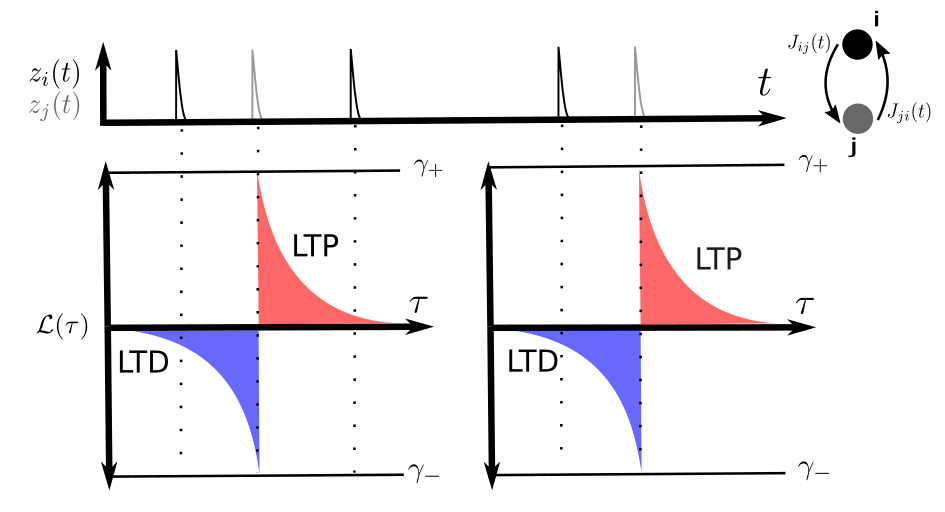
\includegraphics[width=150mm]{figure-5}
\caption{\textbf{Cartoon of the doublet spike-timing dependent plasticity rule}. The time course of two spike trains $z_{i}(t)$ and $z_{j}(t)$ is shown in black and gray, respectively. The learning window $\mathcal{L}(\tau)$ determines whether LTP or LTD occurs and the magnitude of the weight change. Adapted from (Kempter 2001).}
\end{figure}


If we consider only rules that consider the timing of pairs of spikes, changes in synaptic weight can occur from the arrival of a presynaptic spike $z_{i}(t) = 1$, a postsynaptic spike $z_{j}(t) = 1$ or as a function of the delay in spike timing  $\tau$. The spike-timing component of the learning rule is given by the learning window function $\mathcal{L}(\tau)$. A commonly used example of the learning window function is the doublet spike-timing dependent plasticity rule

\begin{align}
\mathcal{L}(\tau) = \begin{cases}
      H(J_{max}-J_{ij})\gamma_{+}\exp(-\tau/\tau_{+}), & \text{if}\ \tau \geq 0 \\
       H(J_{ij})(-\gamma_{-})\exp(-\tau/\tau_{-}), & \text{if} \; \tau < 0
    \end{cases}
\end{align}


which has been illustrated in Fig (1.2). This rule enforces bounds on the weight as well as the sign dependence of the synaptic update characteristic of STDP. Integrating over a time window $\tau_{\mathrm{lrn}}$ gives the total change $\Delta J_{ij}$ (Kempter 1999)


\begin{align}
\Delta J_{ij}(\tau_{\mathrm{lrn}}) &= \int_{0}^{\tau_{\mathrm{lrn}}} dt'\left(a_{i}z_{i}(t') + a_{j}z_{j}(t')\right) \\
&+ \int_{0}^{\tau_{\mathrm{lrn}}} dt'\int_{0}^{\tau_{\mathrm{lrn}}} dt''\mathcal{L}(\tau)z_{i}(t'')z_{j}(t')
\end{align}

The stochasticity of the spike functions $z_{i}(t)$ and $z_{j}(t)$ means that we can only hope to derive the behavior of the above integral on average. In other words, $\Delta J_{ij}$ is itself a stochastic process but we can focus on its drift or expected rate of change. Simulaneously, $z_{i}(t)$ and $z_{j}(t)$ are strongly dependent on the weights $J_{ij}$; however, if the time scale of plasticity is sufficiently long compared to the correlation time scale of the neurons activity, the correlation between $z_{i}(t)$ and $z_{j}(t)$ can be treated as stationary (Kempter 2001). Importantly, the effective correlation time scale of neuron dynamics is intimately related to the timescale over which it is `picked up' by the learning window $\mathcal{L}(\tau)$. Analyzing the drift in $\Delta J_{ij}$ then reads


\begin{align*}
\tau_{\mathrm{lrn}}\frac{\langle \Delta J_{ij}\rangle(t)}{\tau_{\mathrm{lrn}}} &= \int_{0}^{\tau_{\mathrm{lrn}}} dt'\left(a_{i}z_{i}(t') + a_{j}z_{j}(t')\right)\\
&+ \int_{0}^{\tau_{\mathrm{lrn}}} dt'\int_{-t'}^{\tau_{\mathrm{lrn}}-t'} d\tau \mathcal{L}(\tau)\langle z_{i}(t'+\tau)z_{j}(t')\rangle\\
\end{align*}

Note that we can make the same approximations for a sufficiently slow process as we can for a relatively fast process with high time resolution. Then, if synaptic plasticity is sufficiently slow, then we can approximate the average rate of change as $dJ_{ij}/dt \approx \Delta J_{ij}/\tau_{\mathrm{lrn}}$, and the bounds of integration can be set to $-\infty$ and $+\infty$ (Kempter 1999) and we have the final result


\begin{align}
\tau_{\mathrm{lrn}}\frac{d J_{ij}(t)}{dt} &=  a_{i}\langle z_{i}(t)\rangle  + a_{j}\langle z_{j}(t)\rangle + \int_{-\infty}^{+\infty} d\tau \mathcal{L}(\tau)C_{ij}(\tau)
\end{align}

where $\langle z_{i}(t)\rangle$ and $\langle z_{j}(t)\rangle$ can be interpreted as the instantaneous firing rate of neurons $i$ and $j$, respectively. It has already been shown that linear response theory can be used to estimate $C\tau)$ for arbitrary network topologies. Furthermore, the equation (1.22) including the instantaneous post-synaptic firing rate can serve as a homeostatic term if $a_{j} < 0$. Although, as highlighted previously, rate-dependent terms in the learning rule do not selectively enforce LTP and LTD since the term $a_{j}\langle z_{j}(t)\rangle$ appears in the equation for $\dot{J_{ij}}$ for all input neurons $i$ (assuming $a_{j}$ is a constant). Thus we would need to modify (1.22) to arrive at a synaptic plasticity rule which delivers potentiation or depression heterogeneously, for example using information regarding spatial proximity. However, we now argue that this may not be necessary.

\section{Results}

\subsection{Spatial properties of synaptic plasticity}

The integrative properties of neurons depend strongly on the number, proportions and distribution of excitatory and inhibitory synaptic inputs they receive (Megias 2001). Often for the sake of mathematical convenience, models do not account for network structures which have spatial dependence. However, recent experiments have shown that local cortical networks can be dense with connection probabilities sometimes exceeding 40 percent, suggesting a \emph{small-world} organization of neural networks. The conjunction of local clustering and global interaction is thought to provide a structural substrate for the coexistence of functional segregation and integration in the brain (Sporns 2006). 

Furthermore, spatially extended excitatory-inhibitory networks have been rigorously analyzed using techniques from mean-field theory (Rosenbaum 2017). Rosenbaum et al., extended the mean field theory of random networks to prove the existence of a balanced state in networks where connection probabilities obey a Gaussian spatial profile. In this regime, locally dense networks can exhibit irregular firing activity if correlations induced by excitatatory and inhibitory inputs are actively cancelled by a strong negative excitatory-inhibitory correlation. Spatially-extended networks in the balanced state can also exhibit a distinct spatial correlation profile, similar to the correlation profile observed in electrode multielectrode recordings in macaque V1 (Figure 1.3). A similarly shaped spatial profile of long-term plasticity has been observed at the input stage of the cerebellum (Mapelli 2007). Recordings of the activation patterns in the granular layer of the cerebellum upon activation of excitatory and inhibitory mossy fiber projections revealed a bell-shaped excitation profile of the surrounding area. This excitation profile was accompanied by strong inhibition at the periphery of the excited region with the magnitude of inhibition decaying with distance. The sum of excitation and inhibition over space gave a sombrero-shaped profile. Importantly, simultaneous measurements of biomarkers for long term plasticity showed a similar spatial organization of LTP and LTD (Mapelli 2007). That is, regions showing LTP were surrounded by a ring of LTD with little effect at distance regions.  

\begin{figure}[t!]
\centering
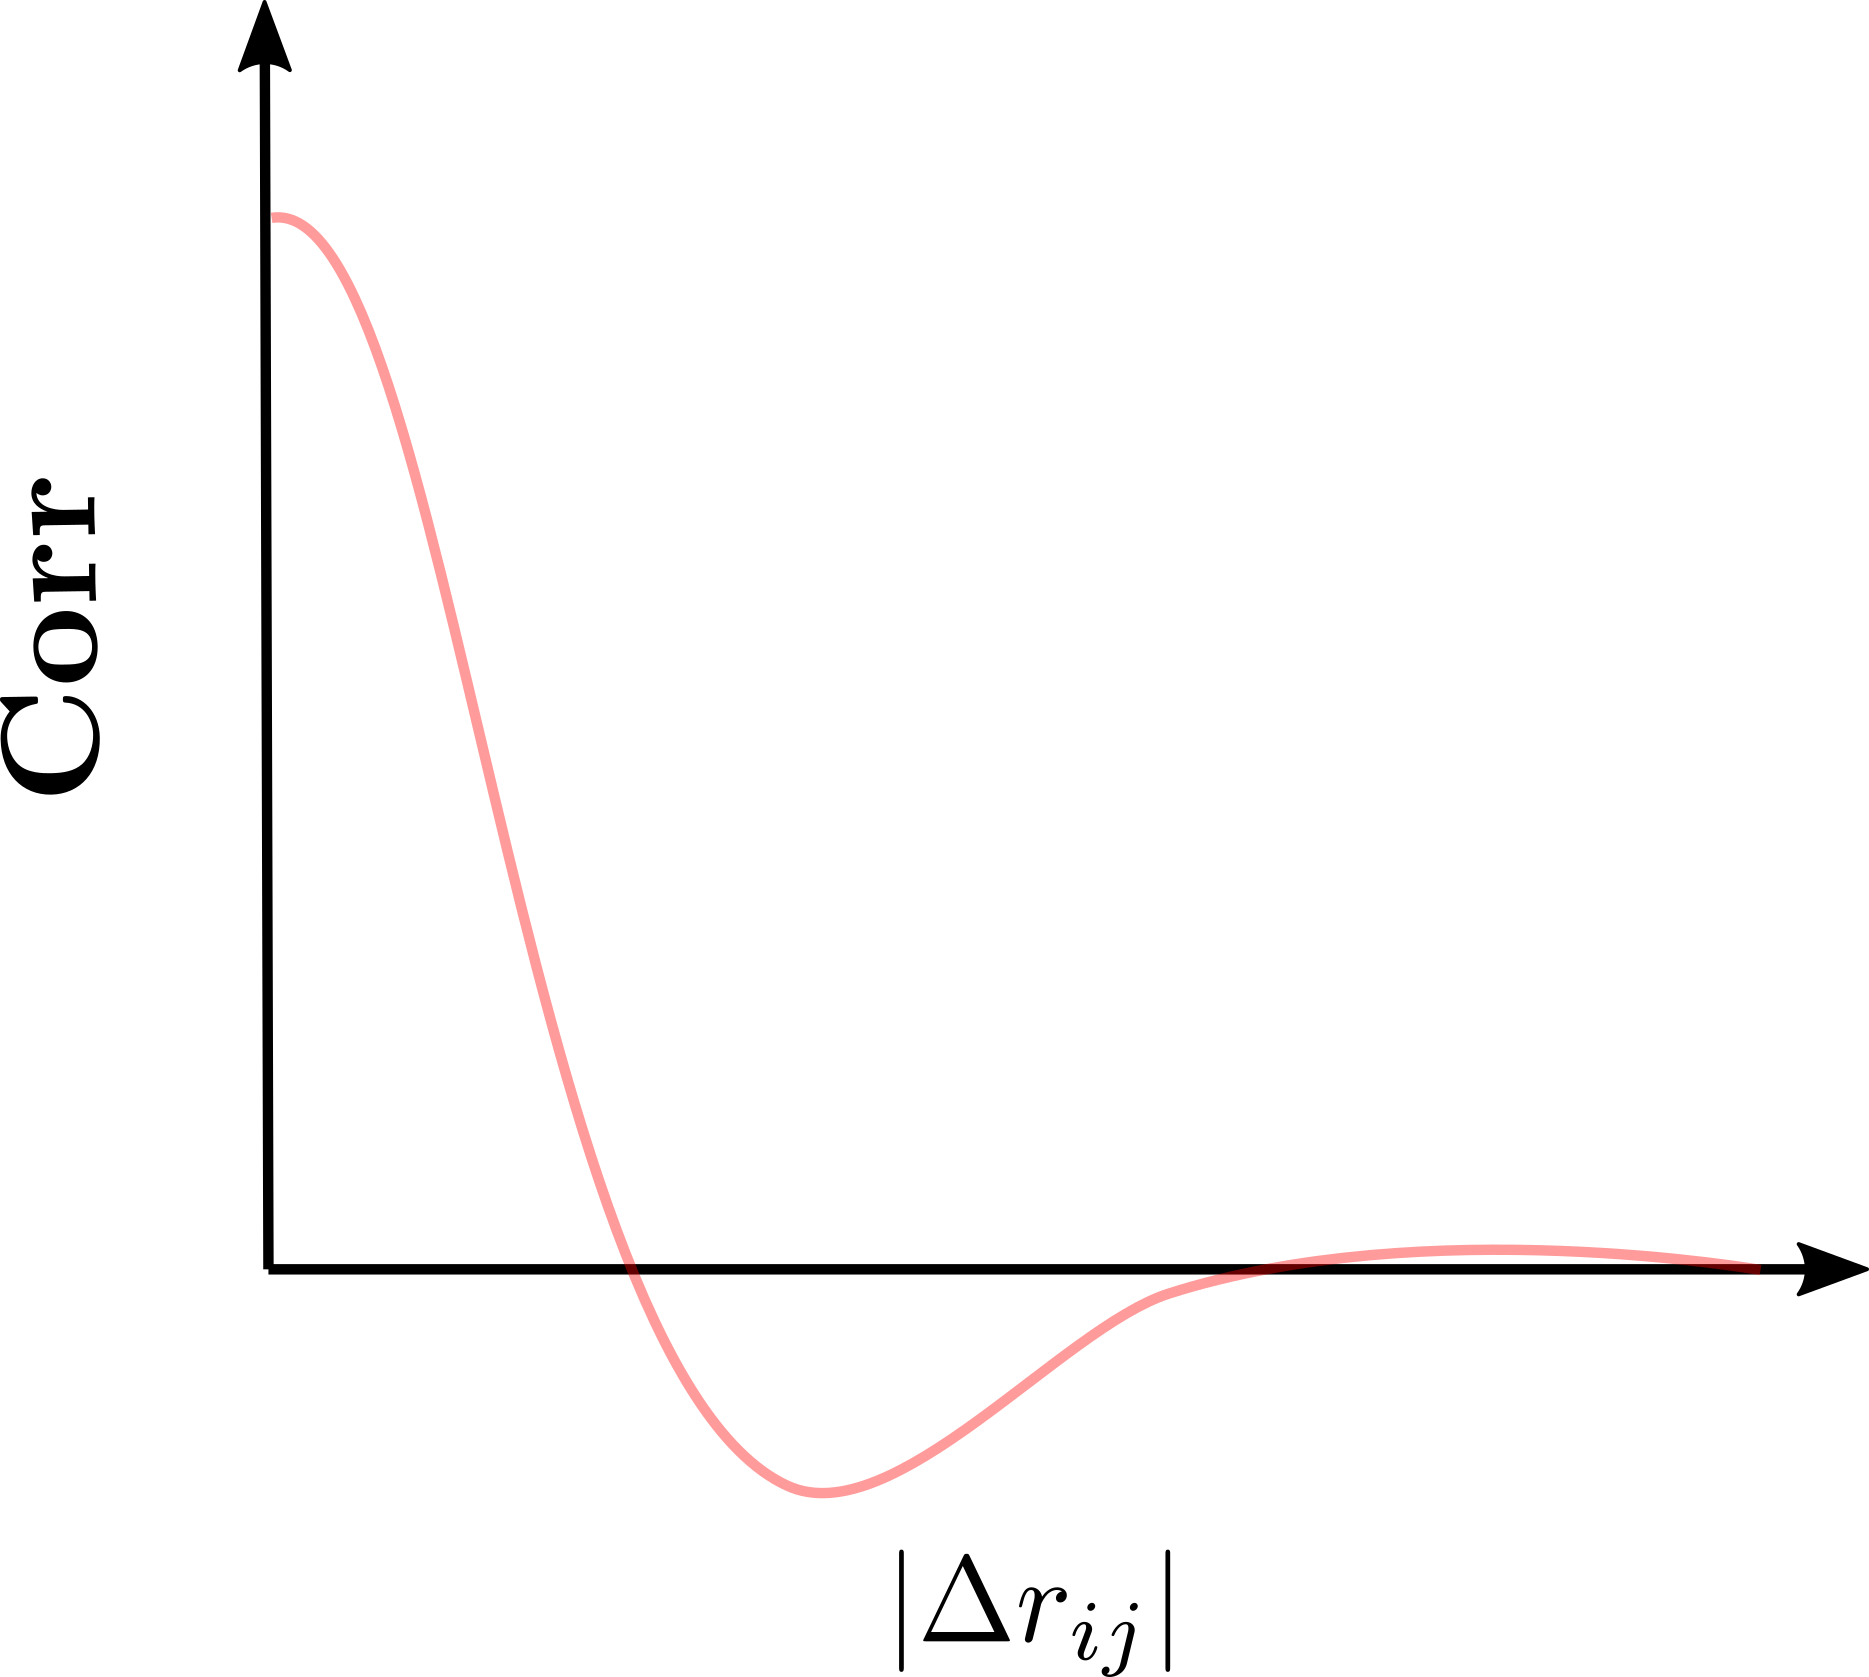
\includegraphics[width=75mm]{figure-10}
\caption{\textbf{Qualitative sketch of the spatial dependence of spike correlations}. Plot shows the spatial profile of correlations that has been measured in balanced spatially-extended networks as well as in electrode recordings of macaque V1.}
\end{figure}

The striking similarity between the spatial correlation structure in simulations of balanced networks and multielectrode recordings could have important implications for cell assembly formation. A spatial-dependence of correlations and long-term plasticity could help drive synaptic competition and synaptic weight normalization. In other words, if the total synaptic conductance a neuron has for its inputs is approximately conserved, the redistribution of conductance could be dependent on spatial proximity. In network models with a logically connected topology, how synaptic conductance should be redistributed is not obvious. Considering then the observation that LTP and LTD can have spatially inhomogeneous properties, we might hypothesize that the balance of excitation and inhibition can result in not only balanced network dynamics but also stability in the formation and maintenance of cell assemblies. An added bonus of this point of view is that predictions on the dynamics of synaptic weights can be expressed theoretically. Using the linear response approximation to predict the matrix of cross-spectra $C(\omega)$ and inserting that prediction into (1.29) gives a coupled set of differential equations for the correlations and the weights. Indeed, that mathematical relationship has already been exploited to make predictions on the dynamics of motifs in an excitatory network (Ocker 2015). Here, a similar formalism is being proposed, except that a special emphasis is placed on the role of excitatory-inhibitory balance in cell assembly formation. 

To begin to answer questions on the relationship of excitatory-inhibitory balance, spike-train correlations, and plasticity effects, the fundamentals of the linear response approximation will first be demonstrated. The following analysis is applied to the simple case of a random network model in the absence of plasticity. This reduction is necessary for two main reasons. First, spike train correlations can be approximated in networks with arbitrary topology; however, proving the existence of a balanced state for an arbitrary topology is not a trivial task. Thus far, proof of a balanced state for spatially-extended networks has been found in a mean-field setting under specific topological constraints. Second, numerical solution of the coupled equations for the synaptic weights and spike-train correlations is a computationally expensive task, especially for large networks. Significant optimization of these numerical methods is needed to address the hypothesis given here.

A very general protocol for solving for the matrix of cross spectra $C(\omega)$ was given in (Trousdale 2012) which can be applied to a network topology of choice. If feedforward currents are uncorrelated, then the solution for $C(\omega)$ simplifies to 

\begin{align}
C(\omega) &= \Delta(\omega)C^{0}(\omega)\Delta^{*}(\omega)
\end{align}

where again the matrix $C^{0}(\omega)$ is again a diagonal matrix of cross-spectra when we do not account for the effect of feedback in the network. 

\subsection{Predicting uncoupled firing rates}

In the linear response framework it is necessary to find the baseline firing rate of neuron from its average input current which is a sum of the mean feedforward input and the mean recurrent input i.e. $\mu = \mu_{F} + \mu_{R}$. Generally, the mean of the feedback current $\mu_{R}$ is found by iteratively solving the Fokker-Planck equation for the specified neuron model and using the predicted firing rate for each neuron to update the rate of the rest of the neurons in the next iteration. That is, at each iteration, we compute

\begin{align*}
\mu_{R}^{t+1} = \mu_{F} + J * r^{t}
\end{align*}

assuming that $\mu_{F}$ is constant. The calculation of average feedback current is expressed in matrix form and $*$ represents standard matrix multiplication. The Fokker-Planck equation is then reparameterized for Gaussian white noise with mean $\mu_{R}^{t+1}$ and variance equal to the variance of the feedforward input. This is referred to as a fixed-point iteration to find the steady state firing rates of all neurons in the network (Trousdale 2012; Ocker 2015). Summarizing the sum of feedforward and feedback currents as a single gaussian variable with mean $\mu_{i}$ gives the following simplified Langevin equation for the membrane potentiial

\begin{align}
\tau\dot{V}_{i}(t) = E - V_{i} + \psi(V_{i}) + \eta_{i}(t)
\end{align}

where $\eta_{i}(t) \sim \mathcal{N}(\mu_{i},\sigma^{2})$. The corresponding Fokker-Planck equation reads

\begin{align}
\frac{\partial P}{\partial t} &= \frac{\sigma^{2}}{\tau}\frac{\partial^{2}P}{\partial V^{2}} + \frac{\partial}{\partial V}\left(\frac{V-E+\psi}{\tau}P\right)
\end{align}

The full details of this method for finding both the steady state density as well as the density under sinusoidal perturbation were given in (Richardson 2007) and will not be repeated here in detail.

\begin{figure}[t!]
\centering
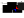
\includegraphics[width=175mm]{figure-3}
\caption{\textbf{Fokker-Planck solution in the uncoupled regime} (A) Steady-state raster plot of $N=100$ uncoupled EIF neurons undergoing stimulation with GWN with $\mu = 2\mu A/\mathrm{cm}^{2}$ and $\sigma = 9 \;\mu A/\mathrm{cm}^{2}$. (B) Histogram of the membrane potential in the steady-state and Fokker-Planck predicted histogram. (C) Two randomly selected voltage traces (D) Histogram of the population-averaged firing rate and its mean value (E) Covariance matrix of the feedforward white-noise input}
\end{figure}

To determine the level of similarity between the numerical prediction of $r_{0}$ versus the result of Monte-Carlo simulations, $N=100$ EIF neurons were simulated for GWN input with $\mu = 2\mu A/\mathrm{cm}^{2}$ and $\sigma = 9 \;\mu A/\mathrm{cm}^{2}$ over a period $T = 1\mathrm{s}$. A spike raster illustrating network activity in the steady state (the last $100\mathrm{ms}$ of the simulation) is shown in Fig (1.4a) with example voltage traces from two randomly selected neurons in Fig (1.4c). The average firing rate measured in simulations was $69.2\mathrm{Hz}$ (Fig 1.4d) in strong agreement with the numerical prediction $73.2\mathrm{Hz}$ (Fig 1.4b). The numerically predicted firing rate can then be used to estimate the frequency spectrum of the spiking activity of each neuron i.e. the value of $C_{ii}^{0}(\omega)$. 

\begin{figure}[t!]
\centering
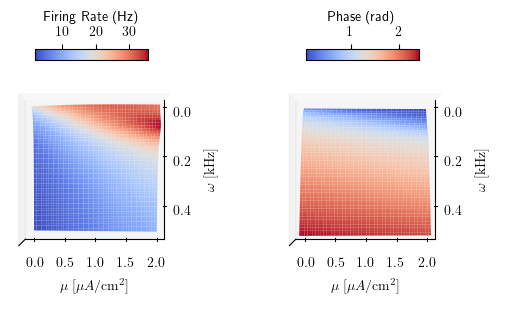
\includegraphics[width=150mm]{figure-4}
\caption{\textbf{Frequency reponse as a function of average input} (left) Predicted firing rate under a weak sinsuoidal perturbation with frequency $\omega$ for various values of the average input current $\mu$. (right) Phase of the response. }
\end{figure}


Next, the frequency response $A_{ii}(\omega)$ was estimated by evaluating the solution of the Fokker-Planck equation for a sinusoidal perturbation. Since, the average input to a neuron $\mu$ will generally depend on the mean value of the feedforward input as well as the rates of other neurons in the network, a solution was found for various values of $\mu$. Interestingly, the magnitude of the frequency response showed a resonance at increasing values of $\omega$ as the average input was increased (Figure 1.5 left). At the same time, the response of the firing rate was in generally in phase with the sinusoidal perturbation for small values of $\omega$ and increasingly out of phase for increasing frequencies. The obtained frequency response, in combination with the estimate of $C_{ii}^{0}(\omega)$ obtained previously from the steady state solution can be used to find an estimate of the solution of (1.31) in later studies when the neurons are coupled.

\begin{figure}[t!]
\centering
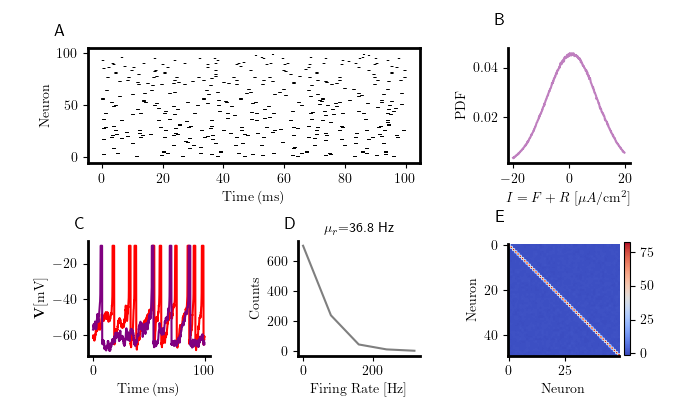
\includegraphics[width=175mm]{figure-11}
\caption{\textbf{Asychronous spiking in the balanced state} (A) Steady-state raster plot of $N=100$ uncoupled EIF neurons undergoing stimulation with GWN with $\mu = 2\mu A/\mathrm{cm}^{2}$ and $\sigma = 9 \;\mu A/\mathrm{cm}^{2}$. (B) Distribution of the total synaptic current in the balanced state (C) Two randomly selected voltage traces (D) Histogram of the population-averaged firing rate and its mean value (E) Covariance matrix of the feedforward GWN input}
\end{figure}


\subsection{Asynchronous spiking in the balanced state}

A central goal of future studies is to make use of mean-field and linear response techniques to generate balanced spatially-extended networks. In particular, it is desirable to use a hybrid approach in which mean-field theory is used to prove the existence of balance and a linear response approximation can detect deviations from the initial balanced state. Moving in this direction, a simple random network model was generated which satisfied the constraints for balance in random networks given previously (see Table 1.2 for a full list of parameters). The synaptic connectivity matrix was taken to be static and synaptic kernels were exponential.  Network stimulation was carried out as before with delta-correlated white noise. Characteristic of the balanced state, the distribution of the sum of feedforward and feedback had zero mean and was bell-shaped. The variance of synaptic current distribution was not examined here, although the result in (Figure 1.6b) suggests that it could be estimated and the Fokker-Planck equation could be used the predict the firing rate. A similar approach has been used for simpler integrate and fire neuron models (Tian 2020). Importantly, the mean firing rate measured was reduced from the uncoupled case by a factor of $\approx 50$ percent, demonstrating the important role of inhibition in preventing runaway firing rates. 


\begin{figure}[t!]
\centering
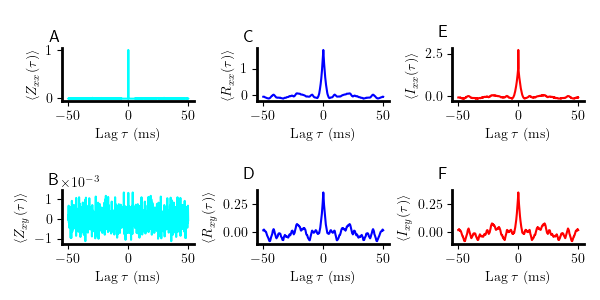
\includegraphics[width=165mm]{figure-12}
\caption{\textbf{Auto- and cross-correlations in the balanced state} (A) Mean auto-correlation of spike trains (B) Mean cross-correlation of spike trains (C) Mean auto-correlation of the feedback current (D) Mean cross-correlation of the feedback current (E) Mean auto-correlation of the total synaptic current (F) Mean cross-correlation of the total synaptic current}
\end{figure}

Auto- and cross-correlations in the balanced state depicted in Fig (1.6) are shown in Fig (1.7). The mean cross-correlation of spike-trains shown as $\langle Z_{xy}(\tau)\rangle$ shows an obvious weak correlation for all $\tau$, as expected in the balanced state. Auto- and cross-correlations for the total synaptic current and its recurrent component appear very similar. This is reasonable, considering that the delta-correlated feedforward input lacks temporal structure and therefore the temporal structure of the total current should be reminiscent of the feedback component. The results of Fig (1.6) and Fig (1.7) are taken as proof of the balanced state in this simple network model. A natural step in a future study would make use of the linear response theory discussed previously to compare these results with theoretical predictions. 

\subsection{A spatially extended network}


In logically-connected networks, the balanced state was achieved by our choice of connection probabilities between excitatory and inhibitory neurons $p_{ee}$, $p_{ie}$, $p_{ei}$ and $p_{ii}$ as well as their respective synaptic weights $j_{ee}$, $j_{ie}$, $j_{ei}$ and $j_{ii}$.  To conclude the present study, a topology in which these probabilities become a function of space will be explored. The network architecture is motivated by the local clustering observed in real neural networks, which has influenced previous theoretical work (Rosenbaum 2017). The network is generated by embedding neurons in a two-dimensional space and the probability of a synapse from a neuron $i$ to neuron $j$ follows a distance-dependent rule with a Gaussian profile

\begin{align}
\Gamma_{ij}(|\Delta\mathbf{r}_{ij}|) = \exp\left(-\frac{1}{2}(\mathbf{r}_{i}-\mathbf{r}_{j})^{T}\mathbf{\Sigma}_{i}(\mathbf{r}_{i}-\mathbf{r}_{j})\right)
\end{align}

with $\mathbf{\Sigma}_{i} = \sigma_{i}^{2}I$. The parameter $\sigma_{i}$ determines the projection width of neuron $i$ and is generally dependent on whether a neuron is excitatory or inhibitory. The existence of excitatory-inhibitory balance will depend strongly on the relative values of $\sigma_{E}$ and $\sigma_{I}$. For a directed network, synapses are then generated by sampling from the following probability distribution 

\begin{equation}
    \mathbb{P} = \left\{\begin{array}{lr}
        p_{ij} = \Gamma_{ij}(1-\Gamma_{ji})(1-q)\cdot Z^{-1}\\
        p_{ji} = \Gamma_{ji}(1-\Gamma_{ij})(1-q)\cdot Z^{-1}\\
        p_{0} = \Gamma_{0}(1-\Gamma_{ij})(1-q)\cdot Z^{-1}\\
        \end{array}\right\}
\end{equation}

\begin{figure}[t!]
\centering
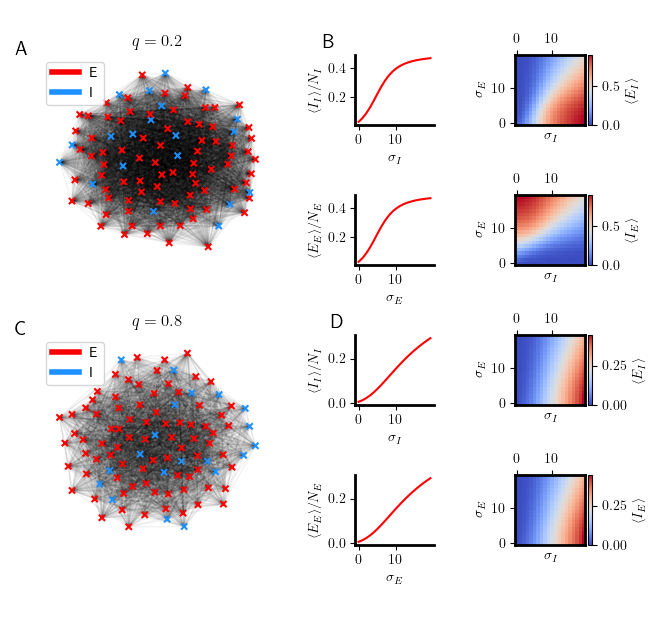
\includegraphics[width=165mm]{figure-9}
\caption{\textbf{Average degree in a spatially-extended exicitatory-inhibitory network} (A) An example dense ($q=0.2$) excitatory-inihbitory network with $N=100$ neurons 80 of which are excitatory. Excitatory neurons are shown in red and inhibitory neurons are shown in blue (C) Average number of synapses in the dense network normalized to the target population size as a function of parameters $\sigma_{E}$ and $\sigma_{I}$. (D) An example sparse excitatory-inihbitory network ($q=0.8$) (E) Average number of synapses in the sparse network normalized to the target population size as a function of parameters $\sigma_{E}$ and $\sigma_{I}$.}
\end{figure}


The dependence of $\Gamma$ on distance has been suppressed for simplicity. Qualitatively, each of these probabilities represent whether a synapse occurs and in what direction. The third probability enforces the overall sparsity in the network and $Z$ is a normalization constant. It is important to note that the in-degree and out-degree distributions of each neuron are not fixed quantities, as they were in Fig (1.6)., which could have important consequences for the existence of a balanced state. To be precise, in previous analyses, the number of inputs of a neuron with type $\alpha$ from a neuron of type $\beta$ was exactly $C_{\alpha\beta} = p_{\alpha\beta}N_{\alpha}$ for every neuron of type $\alpha$. To a first approximation, the existence of excitatory-inhibitory balance in a network where the in-degree is not fixed can be known if the in-degree of the neurons are replaced by their mean values, i.e. $\langle C_{\alpha\beta}\rangle$. However, it remains to be validated whether or not variability in $C_{\alpha\beta}$ can disrupt the balanced state significantly.

To begin to determine if this network topology can exhibit a balanced state, we dissect the degree distribution for both excitatory and inhibitory neurons. The average number of inputs of type $\alpha$ to a neuron of type $\beta$ denoted as $\langle \beta_{\alpha} \rangle$ is simply found by integrating the function $\Gamma$ over the two-dimensional spatial domain (see Methods). The results of this integration are shown in Fig (1.8) for $N=100$ neurons. In principle, we would expect that correlations in this network may arise due to the fact that nearby neurons will tend to have overlapping connections.


\clearpage
\section{Methods}

\subsection{Monte-Carlo simulations}

Monte-Carlo simulations for the balanced random network were run using custom code developed in C and Python. The following exponential integrate and fire (EIF) neuron model was used

\begin{equation}
C\frac{dV_{i}}{dt} = g_{\ell}(E - V_{i}) + g_{\ell}\Delta_{T}\exp\left(\frac{V_{i}-V_{T}}{\Delta_{T}}\right) + R_{i}(t) + \xi_{i}(t)
\end{equation}

with $R(t) = \sum_{i} J_{ij}(t)\cdot \phi(t) * \delta(t-t_{i})$ and $\xi_{i}(t)$ is a delta correlated white noise. The stochastic differential equation (1.30) was integrated numerically using the Euler method and the feedforward input was sampled according to $\xi_{i}(t) \sim \mathcal{N}(\mu_{\mathrm{ext}},\sigma_{\mathrm{ext}}^{2})$. The synaptic kernel was taken to be a decaying exponential i.e. $\phi(t) = \exp(-t/\tau_{s})$. Unless explicitly mentioned otherwise, the parameters for excitatory and inhibitory neurons were kept the same. A full list of parameters used for the balanced random network can be found in Table (1.1). Simulations were run for a total time period $T = 1 \;\mathrm{s}$ with a time resolution of $\Delta t = 100\mathrm{ms}$. Auto- and cross-correlations are calculated by considering the steady state activity which is taken to be the last $100\mathrm{ms}$ of the simulation (this period will be referred to as the steady state window $\Delta t_{ss}$).

Auto- and cross-correlations of feedforward currents, feedback currents, and spike trains were computed by first finding the matrix of cross-spectra $C(\omega)$ using a vectorized Python routine. Before calculating $C(\omega)$, the signals are normalized by subtracting out their mean and dividing by the standard deviation over the steady state window $\Delta t_{ss}$. Let $x(\omega)$ be the discrete-time Fourier transform (DTFT) of an arbitrary signal $x(t)$

\begin{align}
x(\omega) = \sum_{n =-\infty}^{\infty}x(t)\left(\exp{-i\omega n}\right)
\end{align}

We can quickly compute an element matrix of cross-correlations $C_{ij}(\omega)$ in the frequency domain. For example, given spike trains $z_{i}(t)$ and $z_{j}(t)$ we can first apply (1.31) and then take the product

\begin{align}
C_{ij}(\omega) = \underset{T\rightarrow\infty}{\mathrm{lim}}\frac{1}{T}\;z_{i}^{*}(\omega)z_{j}(\omega)
\end{align}

where $*$ represents complex conjugation. The above quantity is the complex-value cross-spectrum of the spike trains $z_{i}(t)$ and $z_{j}(t)$. An identical calculation is carried out for the feedforward, feedback, and total currents.

\subsection{Solution to the Fokker-Planck equation}

As in (1.2), the EIF model uses $\psi(V) = \Delta_{T}\exp\left(\frac{V-V_{T}}{\Delta_{T}}\right)$. (1.33) must be solved for the distribution $P(V_{i},t)$ to find the steady state firing rate of neuron $i$. The basic idea presented in (Richardson 2007) starts with rewriting the Fokker-Planck equation as a continuity equation

\begin{align*}
\frac{\partial P}{\partial t} &= -\frac{\partial J}{\partial V}\\
J &= \frac{\sigma^{2}}{\tau}\frac{\partial P}{\partial V} + \left(\frac{V-E+\psi}{\tau}P\right)
\end{align*}

In the steady state, the second equation above is rearranged to give a coupled set of first order differential equations in the voltage

\begin{align*}
-\frac{\partial P_{0}}{\partial V} &= \frac{\tau}{\sigma^{2}}\left(\frac{V-E+\psi}{\tau}P_{0} + J_{0}\right)\\
-\frac{\partial J_{0}}{\partial V} &= r_{0}\left(\delta(V-V_{\mathrm{th}}) - \delta(V-V_{\mathrm{re}})\right)
\end{align*}

where $V_{\mathrm{th}}$ and $V_{\mathrm{re}}$ refer to the firing threshold and reset potentials, respectively. Briefly, the steady state firing rate $r_{0}$ can be cancelled from the above equations and they can be integrated numerically. Similar expressions exist for the case when the current undergoes a weak sinusoidal perturbation, which is important for finding the linear response function of the firing rate $A(\omega)$. 


\subsection{Generating spatially extended networks}

The method for generating the backbone of the spatially-extended networks in Fig (1.8) will be described. These networks are restricted to be embedded in a discrete two-dimensional space. To generate synapses, a trinomial distribution which determines whether a synapse occurs and its direction is given by

\begin{equation}
    \mathbb{P} = \left\{\begin{array}{lr}
        p_{ij} = \Gamma_{ij}(1-\Gamma_{ji})(1-q)\cdot Z^{-1}\\
        p_{ji} = \Gamma_{ji}(1-\Gamma_{ij})(1-q)\cdot Z^{-1}\\
        p_{0} = \Gamma_{0}(1-\Gamma_{ij})(1-q)\cdot Z^{-1}\\
        \end{array}\right\}
\end{equation}

where $Z$ is a normalization constant and the parameter $q$ is a constant. Neurons are placed on a two-dimensional discrete lattice over which we define a probability kernel $\Gamma_{xx}$ to be a Gaussian function of the separation between two cells

\begin{align}
\Gamma_{ij}(|\Delta\mathbf{r}_{ij}|) = \exp\left(-\frac{1}{2}(\mathbf{r}_{i}-\mathbf{r}_{j})^{T}\mathbf{\Sigma}_{i}(\mathbf{r}_{i}-\mathbf{r}_{j})\right)
\end{align}

To handle the boundary conditions, we take the lattice to be periodic. The distance between any two points on such a lattice is the following Euclidean distance metric

\begin{align*}
|\Delta\mathbf{r}_{ij}|^{2} = \mathrm{min}(|x_1 - x_2|, n\Delta - |x_1 - x_2|)^2 + \mathrm{min}(|y_1 - y_2|, n\Delta - |y_1 - y_2|)^2
\end{align*}


Sampling from the distribution $\mathbb{P}$ for each of the $N^{2} - N$ possible synapses (excluding autapses), we can generate an asymmetric adjacency matrix $\mathcal{C} \in \mathbb{F}_{2}^{N\times N}$. An element $\mathcal{C}_{ij} = 1$ defines a synapse from $i\rightarrow j$ and $\mathcal{C}_{ji} = 1$ defines a synapse from $j\rightarrow i$. Assuming that every synapse is generated independently, the mean of the out-degree distribution is

\begin{equation}
\langle N_{ij} \rangle = \sum_{j} \Gamma_{ij}(1-\Gamma_{ji})(1-\Gamma_{0})\cdot Z^{-1}
\end{equation}

\clearpage
\begin{center}
\captionof{table}{EIF network parameters}
    \begin{tabular}{ | p{4cm} p{7cm} p{4cm} |}
    \hline
    Parameter & Description & Value \\ \hline
    $C$ & Membrane capacitance & 1 $\mu F/\mathrm{cm}^{2}$ \\
    $g_{\ell}$ & Leak conductance & 0.1 $\mathrm{mS}/\mathrm{cm}^{2}$\\
    $V_{\ell}$ & Leak reversal potential & -60 $\mathrm{mV}$ \\
    $\Delta$ & Action pontential steepness & 2 $\mathrm{mV}$ \\
    $V_{T}$ & Action potential initiation threshold & -50 $\mathrm{mV}$ \\
    $V_{\mathrm{th}}$ & Action potential threshold & -10 $\mathrm{mV}$ \\
    $V_{\mathrm{re}}$ & Action potential reset & -60 $\mathrm{mV}$ \\
    $\tau_{\mathrm{ref}}$ & Action potential width & 1.5 $\mathrm{ms}$ \\
    $\mu_{\mathrm{ext}}$ & External input mean & 1 $\mu A/\mathrm{cm}^{2}$ \\
    $\sigma_{\mathrm{ext}}$ & External input s.d. & 9 $\mu A/\mathrm{cm}^{2}$ \\
    $N_{e}$ & Number of excitatory neurons & 500 \\
    $N_{i}$ & Number of inhibitory neurons & 500 \\
    $p_{ee}$ & Probability of $E\rightarrow E$ & 0.25 \\
    $p_{ei}$ & Probability of $E\rightarrow I$ & 0.25 \\
    $p_{ie}$ & Probability of $I\rightarrow E$ & 0.25 \\
    $p_{ii}$ & Probability of $I\rightarrow I$ & 0.25 \\
    $j_{ee}$ & Weight of $E\rightarrow E$ & 12.5 $\mu A/\mathrm{cm}^{2}$ \\
    $j_{ei}$ & Weight of $I\rightarrow E$ & 50 $\mu A/\mathrm{cm}^{2}$\\
    $j_{ie}$ & Weight of $E\rightarrow I$ & 20 $\mu A/\mathrm{cm}^{2}$ \\
    $j_{ii}$ & Weight of $I\rightarrow I$ & 50 $\mu A/\mathrm{cm}^{2}$\\
    $\tau_{s}$ & Excitatory synaptic time constant & 4 $\mathrm{ms}$\\
    \hline

    \end{tabular}
\end{center}


%% Format a LaTeX bibliography

\makebibliography

\noindent [1] Buesing et al. \textit{Neural dynamics as sampling: A model for stochastic computation in recurrent networks of spiking neurons}.           PLoS Computational Biology 2011.
\newline
\noindent [2] Azouz et al. \textit{Cellular Mechanisms Contributing to Response Variability of Cortical Neurons In Vivo}. Journal of Neuroscience. 1999.
\newline
\noindent [3] Vreeswijk et al. \textit{Chaotic Balanced State in a Model of Cortical Circuits}. Neural Computation. 1998.
\newline
\noindent [4] Rosenbaum et al. \textit{The spatial structure of correlated neuronal variability}. Nature Neuroscience. 2017.
\newline
\noindent [5] M.E. Richardson. \textit{Firing-rate response of linear and nonlinear integrate-and-fire neurons to modulated current-based and conductance-based synaptic drive}. Physical Review E. 2007
\newline
\noindent [6] Ocker et al. \textit{Self-Organization of Microcircuits in Networks of Spiking Neurons with Plastic Synapses}. PLoS Computational Biology. 2015.
\newline
\noindent [7] Ocker et al. \textit{Linking structure and activity in nonlinear spiking networks}. PLoS Computational Biology. 2017.
\newline
\noindent [8] D.O. Hebb \textit{The organization of behavior; a neuropsychological theory}. Wiley Publishing. 1949.
\newline
\noindent [9] Kumar et al. \textit{Formation and maintenance of neuronal assemblies through synaptic plasticity}. Nature Communications. 2014.
\newline
\noindent [10] Cohen et al. \textit{Measuring and interpreting neuronal correlations}. Nature Neuroscience. 2011.
\newline
\noindent [11] Ostojic et al. \textit{How connectivity, background activity, and synaptic properties shape the cross-correlation between spike trains}. Journal of Neuroscience. 2009.
\newline
\noindent [12] Ostojic et al. \textit{How connectivity, background activity, and synaptic properties shape the cross-correlation between spike trains}. Journal of Neuroscience. 2009.
\newline
\noindent [13] Csicsvari et al. \textit{Reliability and State Dependence of Pyramidal Cell–Interneuron Synapses in the Hippocampus: an Ensemble Approach in the Behaving Rat}. Neuron. 1998.
\newline
\noindent [14] Faisa et al.. \textit{Noise in the nervous system}. Nature Reviews Neuroscience. 2008.
\newline
\noindent [15] Vreeswijk et al. \textit{Chaos in Neuronal Networks with Balanced Excitatory and Inhibitory Activity}. Science. 2008.
\newline
\noindent [16] Baker et al. \textit{Correlated states in balanced neuronal networks}. Physical Review E. 2019.
\newline
\noindent [17] Tetzlaff et al. \textit{Decorrelation of Neural-Network Activity by Inhibitory Feedback}. PLoS Computational Biology. 2012.
\newline
\noindent [18] Doiron et al. \textit{The mechanics of state-dependent neural correlations}. Nature Neuroscience. 2016.
\newline
\noindent [19] Tian et al. \textit{Excitation-inhibition balanced neural networks for fast signal detection}. Frontiers in Computational Neuroscience. 2020.
\newline
\noindent [20] Plesser et al. \textit{Noise in integrate and fire neurons: from stochastic inputs to escape rates}. Neural Computation. 2000.
\newline
\noindent [21] Plesser et al. \textit{Noise in integrate and fire neurons: from stochastic inputs to escape rates}. Neural Computation. 2000.
\newline
\noindent [22] Kempter et al. \textit{How the threshold of a neuron determines its capacity for coincidence detection}. Biosystems. 1998.
\newline
\noindent [23] Renart et al. \textit{The Asynchronous State in Cortical Circuits}. Science. 2010.
\newline
\noindent [24] Akil et al. \textit{Balanced networks under spike-time dependent plasticity}. PLoS Computational Biology. 2021.
\newline
\noindent [25] Song et al. \textit{Highly Nonrandom Features of Synaptic Connectivity in Local Cortical Circuits}. PLoS Biology. 2005.
\newline
\noindent [26] Lindner et al. \textit{Theory of oscillatory firing induced by spatially correlated noise and delayed inhibitory feedback}. Physical Review E. 2005.
\newline
\noindent [27] Trousdale et al. \textit{Impact of Network Structure and Cellular Response on Spike Time Correlations}. PLoS Computational Biology. 2012.
\newline
\noindent [28] N. Brunel. \textit{Dynamics of Sparsely Connected Networks of Excitatory and Inhibitory Spiking Neurons}. Journal of Computational Neuroscience. 2000.
\newline
\noindent [29] Brunel et al. \textit{Fast global oscillations in networks of integrate-and-fire neurons with low firing rates}. Neural Computation. 1999.
\newline
\noindent [30] Brunel et al. \textit{Theory of Input Spike Auto- and Cross-Correlations and Their Effect on the Response of Spiking Neurons}. Neural Computation. 2008.
\newline
\noindent [31] DeWeese et al. \textit{Non-Gaussian Membrane Potential Dynamics Imply Sparse, Synchronous Activity in Auditory Cortex}. Journal of Neuroscience. 2006.
\newline
\noindent [32] Buzaki et al. \textit{Neural syntax: cell assemblies, synapsembles and readers}. Neuron. 2010.
\newline
\noindent [33] Mongillo et al. \textit{Synaptic Theory of Working Memory}. Science. 2008.
\newline
\noindent [34] Whitlock et al. \textit{Learning induces long-term potentiation in the hippocampus}. Science. 2006.
\newline
\noindent [35] Bliss et al. \textit{Long-lasting potentiation of synaptic transmission in the dentate area of the anaesthetized rabbit following stimulation of the perforant path}. Journal of Physiology. 1973.
\newline
\noindent [36] Markram et al. \textit{Regulation of synaptic efficacy by coincidence of postsynaptic APs and EPSPs}. Science. 1997.
\newline
\noindent [37] Song et al. \textit{Competitive Hebbian learning through spike-timing-dependent synaptic plasticity}. Nature Neuroscience. 2000.
\newline
\noindent [38] Song et al. \textit{Competitive Hebbian learning through spike-timing-dependent synaptic plasticity}. Nature Neuroscience. 2000.
\newline
\noindent [39] Sjostrom et al. \textit{Rate, timing, and cooperativity jointly determine cortical synaptic plasticity}. Neuron. 2001.
\newline
\noindent [40] Sumi et al. \textit{Mechanism underlying hippocampal long-term potentiation and depression based on competition between endocytosis and exocytosis of AMPA receptors}. Scientific Reports. 2020.
\newline
\noindent [41] Lisman et al. \textit{A mechanism for the Hebb and the anti-Hebb processes underlying learning and memory}. PNAS. 1989.
\newline
\noindent [42] Nabavi et al. \textit{Metabotropic NMDA receptor function is required for NMDA receptor-dependent long-term depression}. PNAS. 2013.
\newline
\noindent [43] Royer et al. \textit{Conservation of total synaptic weight through balanced synaptic depression and potentiation}. Nature. 2003.
\newline
\noindent [44] Morrison et al. \textit{Spike-timing-dependent plasticity in balanced random networks}. Neural Computation. 2007.
\newline
\noindent [45] Megias et al. \textit{Total number and distribution of inhibitory and excitatory synapses on hippocampal CA1 pyramidal cells}. Neuroscience. 2001.
\newline
\noindent [46] Sporns. \textit{Small worlds inside big brains}. PNAS. 2006.
\newline
\noindent [47] Mapelli. \textit{The Spatial Organization of Long-Term Synaptic Plasticity at the Input Stage of Cerebellum}. Journal of Neuroscience. 2007.
\newline





\end{document}


